% Regenerate with latex and dvisvgm; see graph-matching-common.tex.
% Shared styles for the vector replacements in graph-matching/.
% Compile each diagram from this directory, for example:
% latex -interaction=nonstopmode -halt-on-error augment-1.tex
% dvisvgm --no-fonts --exact --bbox=papersize -o augment-1.svg augment-1.dvi
\documentclass[tikz,border=5pt]{standalone}
\usepackage{lmodern,amssymb}
\usetikzlibrary{arrows.meta,backgrounds,calc}
\definecolor{matchred}{HTML}{D7191C}
\definecolor{matchblue}{HTML}{1748B5}
\definecolor{blossomgreen}{HTML}{087A16}
\definecolor{blossomfill}{HTML}{B3E3AF}
\tikzset{
  diagram/.style={x=1mm,y=-1mm,font=\small,line width=.6pt,
    line cap=round,line join=round,
    background rectangle/.style={fill=white},show background rectangle},
  vertex/.style={circle,draw,fill=white,minimum size=5mm,inner sep=0pt},
  point/.style={circle,fill=black,minimum size=2.8mm,inner sep=0pt},
  exposed/.style={point,draw=matchred,fill=matchred!80,line width=1pt},
  matching/.style={line width=2pt},
  transition/.style={-{Stealth[length=4mm,width=3mm]},
    line width=1.4pt,draw=matchblue},
  blossom/.style={draw=blossomgreen,fill=blossomfill,line width=1pt},
  route/.style={draw=matchred,line width=.9pt},
  label/.style={inner sep=1.5pt,align=center},
}

% The five-cycle has exactly two matching edges. Its exposed base is b0.
% Call inside a scope to translate the entire blossom consistently.
\newcommand{\FiveBlossom}{%
  \draw[blossom] (16,0) circle[radius=22mm];
  \foreach \id/\px/\py in {b0/0/0,b1/12/-16,b2/29/-9,b3/29/10,b4/11/16}
    \node[point] (\id) at (\px,\py) {};
  \draw (b0) -- (b1) (b2) -- (b3) (b4) -- (b0);
  \draw[matching] (b1) -- (b2) (b3) -- (b4);
  \node[label,text=blossomgreen,above] at (16,-22) {blossom};
  \node[label,text=blossomgreen,above=.3mm,xshift=-2mm] at (b0.north) {root};
  \node[label,below=.5mm] at (b0.south) {$v$};
}

\begin{document}
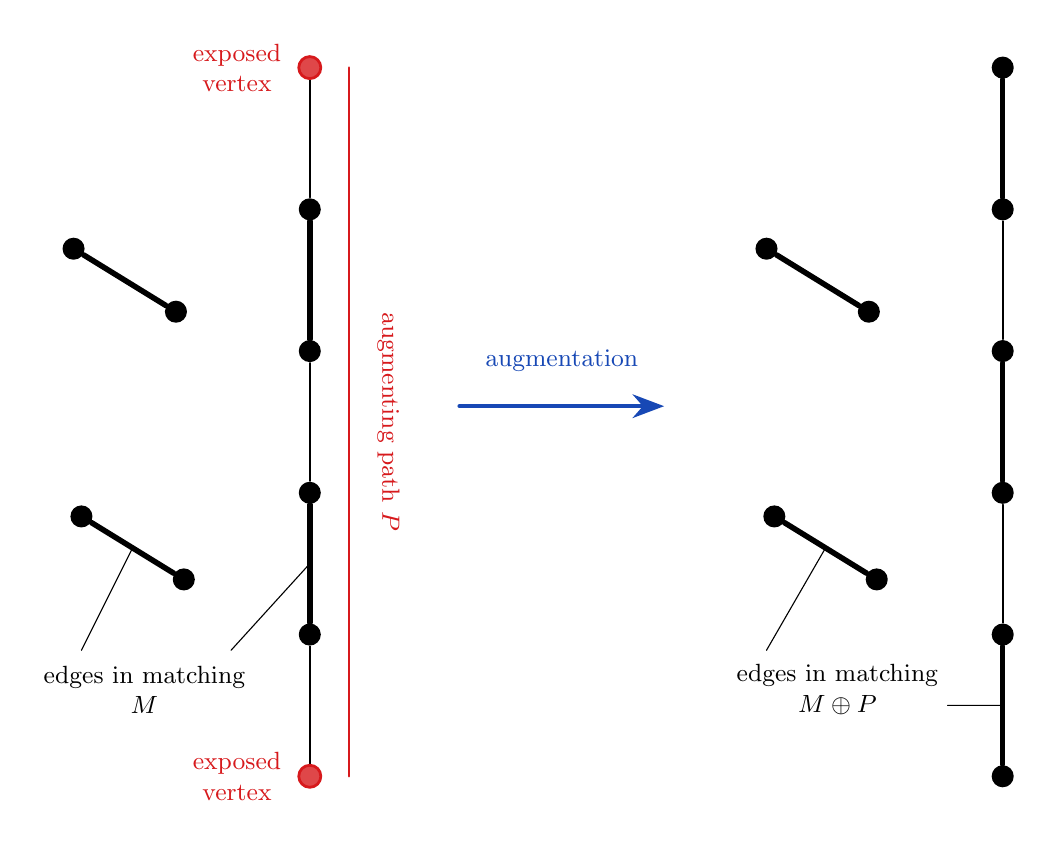
\begin{tikzpicture}[diagram]
  % P has six vertices and five alternating edges. The two isolated
  % matching edges outside P are retained in both panels, as in the PNG.
  % Only the matching edges on P change, from two to three.
  \foreach \panel/\offset in {before/0,after/88} {
    \begin{scope}[xshift=\offset mm]
      \foreach \i in {0,...,5}
        \node[point] (\panel-\i) at (0,18*\i) {};
      \foreach \i/\j in {0/1,1/2,2/3,3/4,4/5}
        \draw (\panel-\i) -- (\panel-\j);
      \foreach \i/\px/\py in {0/-30/23,1/-17/31,2/-29/57,3/-16/65}
        \node[point] (\panel-off-\i) at (\px,\py) {};
      \draw[matching] (\panel-off-0) -- (\panel-off-1)
        (\panel-off-2) -- (\panel-off-3);
    \end{scope}
  }
  \draw[matching] (before-1) -- (before-2) (before-3) -- (before-4);
  \draw[matching] (after-0) -- (after-1) (after-2) -- (after-3)
    (after-4) -- (after-5);
  \foreach \i in {0,5} {
    \node[exposed] at (before-\i) {};
    \node[label,text=matchred,left=3mm] at (before-\i) {exposed\\vertex};
  }
  \draw[route] (5,0) -- (5,90);
  \node[label,text=matchred,rotate=-90] at (10,45) {augmenting path $P$};
  \draw[transition] (19,43) -- (45,43)
    node[midway,above=3mm,text=matchblue] {augmentation};
  \node[label] at (-21,79) {edges in matching\\$M$};
  \node[label] at (67,79) {edges in matching\\$M\oplus P$};
  \draw[line width=.4pt] (-29,74) -- ($(before-off-2)!.5!(before-off-3)$)
    (-10,74) -- ($(before-3)!.5!(before-4)$);
  \draw[line width=.4pt] (58,74) -- ($(after-off-2)!.5!(after-off-3)$)
    (81,81) -- ($(after-4)!.5!(after-5)$);
\end{tikzpicture}
\end{document}
